\section{ODD for StationSim GCS}
\label{sec:stationsim}

\subsection{Overview}
\label{sub:stationsim:overview}

\subsubsection{Purpose and patterns}
\label{subs:stationsim:overview:purpose}

StationSim GCS is an updated version of the StationSim model.
The original StationSim aimed to simulate the motion of pedestrians across a
hypothetical rectangular station with 3 entrances on one side and 2 exits on the
opposite side as shown in Figure \ref{fig:stationsim_env}.
The new StationSim GCS also aims to simulation the motion of pedestrians across
a station; however, in this case the model is based on the real-world example of
Grand Central Station in New York, focusing specifically on the concourse area
highlighted in Figure \ref{fig:gcs_concourse}.
This is reflected in the simulation environment shown in Figure
\ref{fig:stationsim_gcs_env}.
The environment consists of X gates which act simultaneously as both entrances
and exits.
Each pedestrian in the simulation is assigned an entrance and an exit and, upon
entering the environment, seeks to move as directly as possible towards their
assigned exit without colliding with other pedestrians.
Where collisions are more likely to occur (e.g. close to entrances/exits and
around solid obstacles), we typically observe crowding as population densities
increase.

\begin{figure}[h]
    \centering
    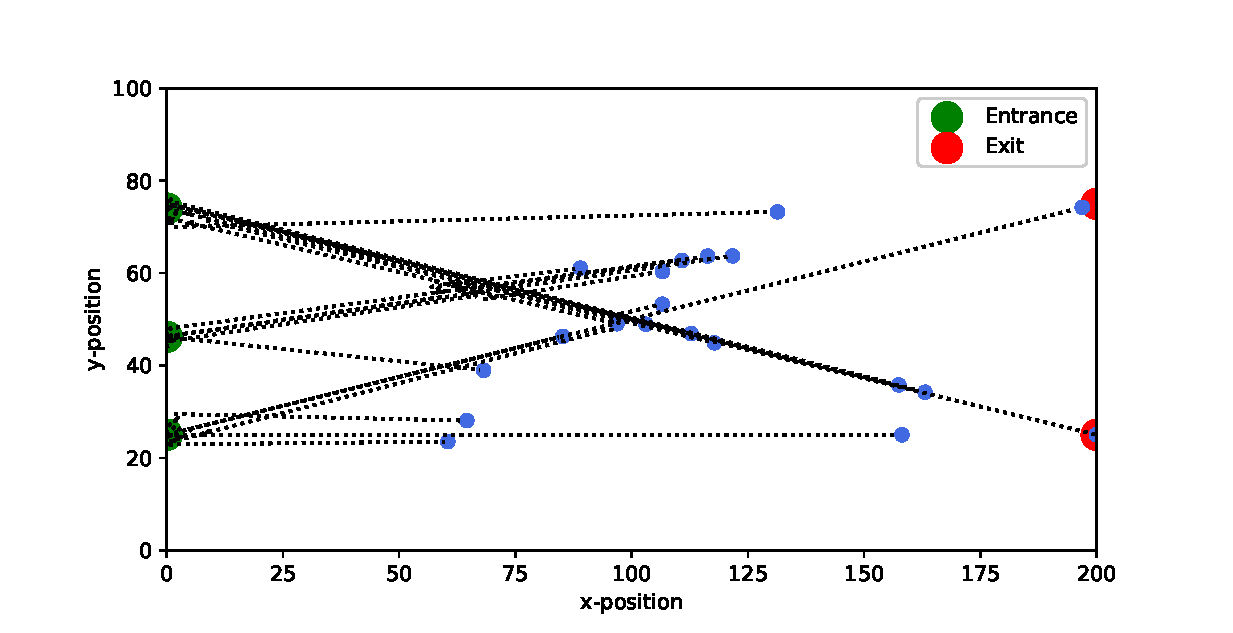
\includegraphics[width=0.7\textwidth]{sample_model_run}
    \caption{Layout of environment in original StationSim model.}
    \label{fig:stationsim_env}
\end{figure}

\begin{figure}[h]
    \centering
    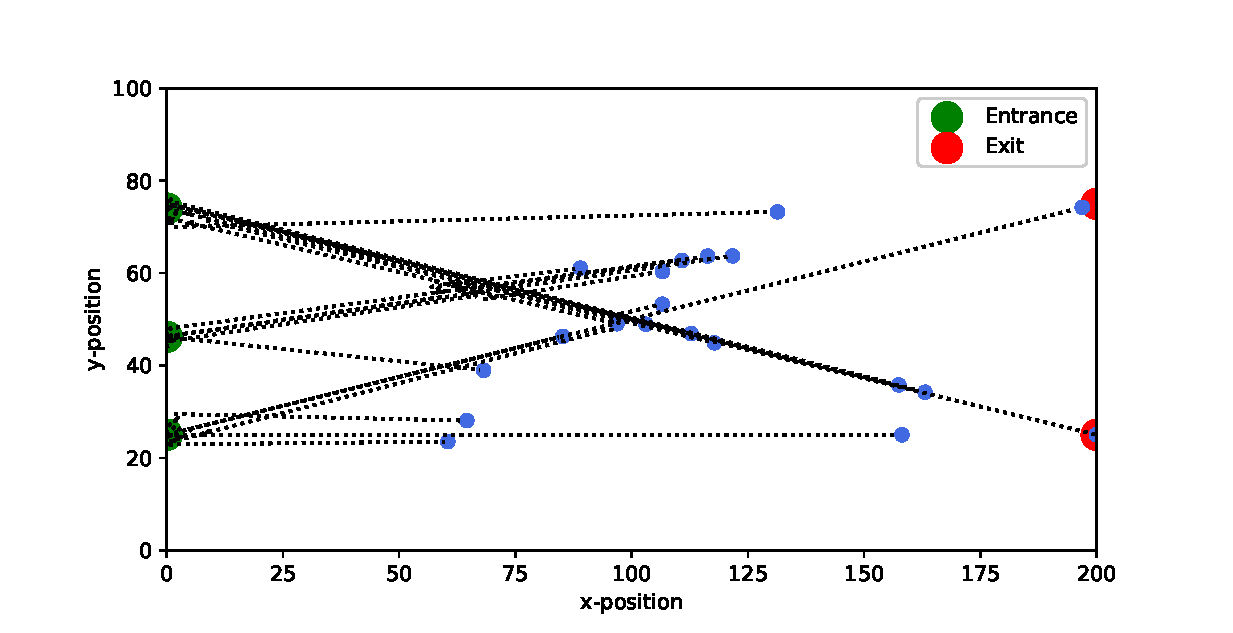
\includegraphics[width=0.7\textwidth]{sample_model_run}
    \caption{Layout of Grand Central Station concourse.}
    \label{fig:gcs_concourse}
\end{figure}

\begin{figure}[h]
    \centering
    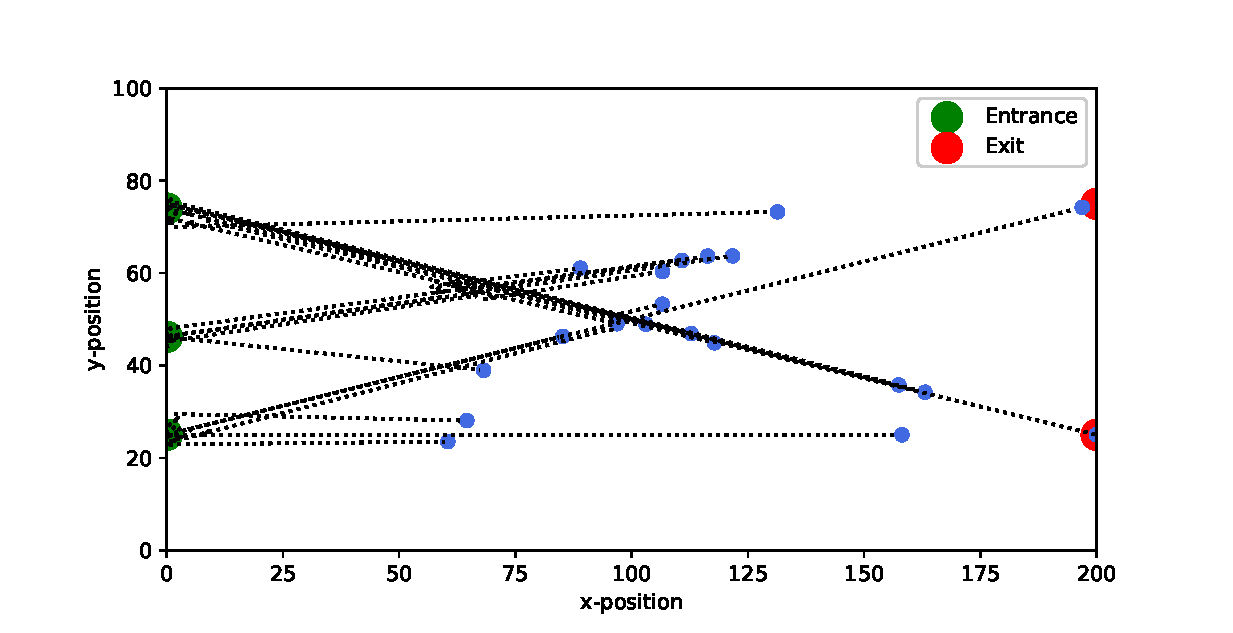
\includegraphics[width=0.7\textwidth]{sample_model_run}
    \caption{Layout of environment in StationSim GCS model.}
    \label{fig:stationsim_gcs_env}
\end{figure}

\subsubsection{Entities, state variables and scales}
\label{subs:stationsim:overview:entities}

The StationSim GCS model consists of agents representing pedestrians moving
around an environment.
Agent attributes are detailed in Table X.


INSERT TABLES OF VARIABLES

\begin{itemize}
    \item Agents
    \begin{itemize}
        \item
    \end{itemize}
    \item Gates
    \begin{itemize}
        \item
    \end{itemize}
    \item Environment
    \begin{itemize}
        \item
    \end{itemize}
    \item Obstacles
    \begin{itemize}
        \item
    \end{itemize}
\end{itemize}

\subsubsection{Process overview and scheduling}
\label{subs:stationsim:overview:process}

INSERT FLOW DIAGRAM OF OVERARCHING PROCESS OF MODEL

\subsection{Design Concepts}
\label{sub:stationsim:design_concepts}

\begin{enumerate}
    \item Basic principles
    \item Emergence
    \item Adaptation
    \item Objectives
    \item Learning
    \item Prediction
    \item Sensing
    \item Interaction
    \item Stochasticity
    \item Collectives
    \item Observation
\end{enumerate}

\subsection{Details}
\label{sub:stationsim:details}

\subsubsection{Initialisation}
\label{subs:stationsim:details:initialisation}

\subsubsection{Input data}
\label{subs:stationsim:details:input}

\subsubsection{Submodels}
\label{subs:stationsim:details:submodels}

